\documentclass[
11pt, % The default document font size, options: 10pt, 11pt, 12pt
%codirector, % Uncomment to add a codirector to the title page
]{charter} 


% El títulos de la memoria, se usa en la caratula y se puede usar el cualquier lugar del documento con el comando \ttitle
\titulo{Sistema de monitoreo de \textit{Rhynchophorus ferrugineus} en palmeras de Montevideo} 


% Nombre del posgrado, se usa en la caratula y se puede usar el cualquier lugar del documento con el comando \degreename
% \posgrado{Carrera de Especialización en Sistemas Embebidos} 
%\posgrado{Carrera de Especialización en Internet de las Cosas} 
\posgrado{Carrera de Especialización en Inteligencia Artificial}
%\posgrado{Maestría en Sistemas Embebidos} 
%\posgrado{Maestría en Internet de las cosas}

% Tu nombre, se puede usar el cualquier lugar del documento con el comando \authorname
% IMPORTANTE: no omitir titulaciones ni tildación en los nombres, también se recomienda escribir los nombres completos (tal cual los tienen en su documento)
\autor{Ing. Bruno Masoller}

% El nombre del director y co-director, se puede usar el cualquier lugar del documento con el comando \supname y \cosupname y \pertesupname y \pertecosupname
\director{Ing. Juan Ignacio Cavalieri}
\pertenenciaDirector{FIUBA} 
\codirector{} % para que aparezca en la portada se debe descomentar la opción codirector en los parámetros de documentclass
\pertenenciaCoDirector{FIUBA}

% Nombre del cliente, quien va a aprobar los resultados del proyecto, se puede usar con el comando \clientename y \empclientename
\cliente{Ing. Agr. Alfonso Arcos}
\empresaCliente{Intendencia de Montevideo}
 
\fechaINICIO{15 de octubre de 2024}		%Fecha de inicio de la cursada de GdP \fechaInicioName
\fechaFINALPlan{03 de diciembre de 2024} 	%Fecha de final de cursada de GdP
\fechaFINALTrabajo{junio de 2025}	%Fecha de defensa pública del trabajo final


\begin{document}

\maketitle
\thispagestyle{empty}
\pagebreak


\thispagestyle{empty}
{\setlength{\parskip}{0pt}
  \tableofcontents{}
}
\pagebreak

\section*{Registros de cambios}
\label{sec:registro}


\begin{table}[ht]
  \label{tab:registro}
  \centering
  \begin{tabularx}{\linewidth}{@{}|c|X|c|@{}}
    \hline
    \rowcolor[HTML]{C0C0C0}
    Revisión & \multicolumn{1}{c|}{\cellcolor[HTML]{C0C0C0}Detalles de los cambios realizados}       & Fecha                       \\ \hline
    0        & Creación del documento                                                                & \fechaInicioName            \\ \hline
    1        & Se completa hasta el punto 5 inclusive                                                & {29} de {octubre} de 2024   \\ \hline
    2        & Se corrige secciones 1, 2, 3, 4 y 5. \newline Se completa hasta el punto 9 inclusive. & {05} de {noviembre} de 2024 \\ \hline
    3        & Se corrige secciones 1, 2, 6 y 9. \newline Se completa hasta el punto 12 inclusive.   & {12} de {noviembre} de 2024 \\ \hline
    4        & Se corrige secciones 1, 9 y 12. \newline Se completa el plan.                         & {19} de {noviembre} de 2024 \\ \hline

    % Si hay más correcciones pasada la versión 4 también se deben especificar acá
  \end{tabularx}
\end{table}

\pagebreak

\section*{Acta de constitución del proyecto}
\label{sec:acta}

\begin{flushright}
  Buenos Aires, \fechaInicioName
\end{flushright}

\vspace{2cm}

Por medio de la presente se acuerda con el \authorname\hspace{1px} que su Trabajo Final de la \degreename\hspace{1px} se titulará ``\ttitle'' y consistirá en la presentación de una prueba de concepto de un sistema de monitoreo de la plaga \textit{Rhynchophorus ferrugineus} en palmeras de Montevideo. El trabajo tendrá un presupuesto preliminar estimado de 600 horas y un costo estimado de USD 30156, con fecha de inicio el \fechaInicioName\hspace{1px} y fecha de presentación pública en \fechaFinalName.

Se adjunta a esta acta la planificación inicial.

\vfill

% Esta parte se construye sola con la información que hayan cargado en el preámbulo del documento y no debe modificarla
\begin{table}[ht]
  \centering
  \begin{tabular}{ccc}
    \begin{tabular}[c]{@{}c@{}}Dr. Ing. Ariel Lutenberg \\ Director posgrado FIUBA\end{tabular} & \hspace{2cm} & \begin{tabular}[c]{@{}c@{}}\clientename \\ \empclientename \end{tabular} \vspace{2.5cm} \\
    \multicolumn{3}{c}{\begin{tabular}[c]{@{}c@{}} \supname \\ Director del Trabajo Final\end{tabular}} \vspace{2.5cm}                                                                                   \\
  \end{tabular}
\end{table}

\section{1. Descripción técnica-conceptual del proyecto a realizar}
\label{sec:descripcion}

En Montevideo, hay alrededor de 25.000 palmeras, que forman una parte esencial del paisaje urbano y contribuyen al equilibrio del ecosistema local. Desde 2010, la plaga del \textit{Rhynchophorus ferrugineus}, conocido comúnmente como “picudo rojo” (ver figura \ref{fig:picudo-rojo}), ha estado propagándose por América, llegando a Uruguay en 2022. Esta plaga supone una amenaza grave para las palmeras, ya que las larvas de este escarabajo se alimentan de su tejido interno, causando el colapso estructural de los árboles en un período de entre 8 y 10 meses.

La infestación del picudo rojo no solo tiene consecuencias ecológicas, sino también económicas. La caída de palmeras infectadas puede provocar daños a personas y propiedades, especialmente durante los fuertes vientos que afectan a Montevideo. Además, la eliminación de estos árboles infestados implica un costo aproximado de 1.000 dólares estadounidenses por unidad.

\begin{figure}[H]
  \centering
  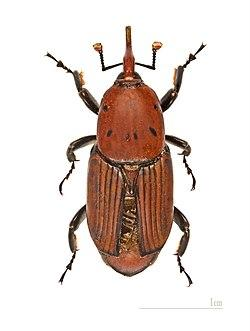
\includegraphics[width=.30\textwidth]{./Figuras/picudo-rojo.png}
  \caption{Rhynchophorus ferrugineus.}
  \label{fig:picudo-rojo}
\end{figure}

Actualmente, el método principal método de detección que utiliza la Intendencia de Montevideo (IM), consiste en la inspección visual presencial en lugares donde se sospecha la presencia de la plaga o se ha reportado por parte de particulares. La IM también tiene otros métodos de detección, como lo son trampas colocadas en puntos claves de la ciudad que permiten observar el desplazamiento de la plaga.

El servicio de Áreas Verdes es el principal encargado del tratamiento de la plaga del picudo rojo y gestiona sectores clave, como el de arbolado, que representa una de las primeras líneas de defensa. Este servicio proporciona diversos datos y colabora estrechamente con otras áreas importantes para la gestión de la plaga, como los servicios de Geomática e Informática. Entre los datos disponibles, se incluye la ubicación de todas las palmeras en el sistema de información geográfica de la IM. Además, el servicio de Geomática cuenta con drones que permiten obtener imágenes de ortomosaicos bajo demanda (ver figura \ref{fig:imagen-dron-y-avion}), las cuales pueden ser solicitadas por el servicio de Áreas Verdes. Estos ortomosaicos alcanzan una resolución espacial de 3 cm por píxel en el rango espectral RGB. Adicionalmente, se realizan vuelos que cubren toda la ciudad de Montevideo, lo cual permite la generación de ortomosaicos de alta resolución en dicho rango espectral.

\begin{figure}[H]
  \centering
  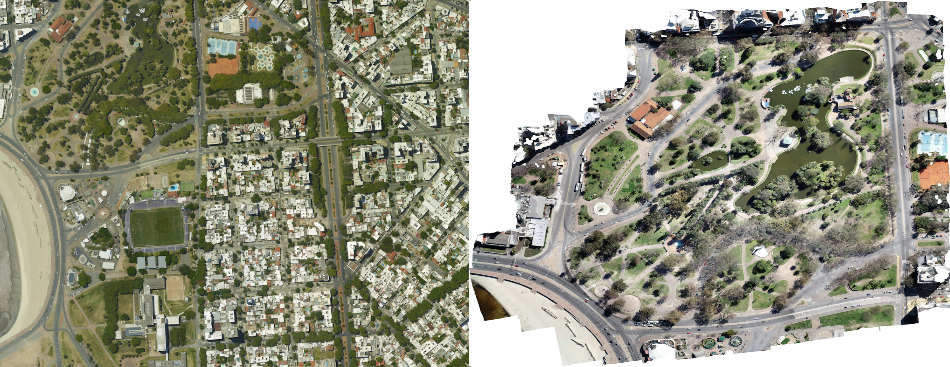
\includegraphics[width=.95\textwidth]{./Figuras/imagen-dron-y-avion.png}
  \caption{Fotografías ortorectificadas de un vuelo de avión y dron, respectivamente.}
  \label{fig:imagen-dron-y-avion}
\end{figure}

Se ha demostrado la viabilidad de detectar la plaga utilizando imágenes capturadas con Google Street View (a nivel de suelo) \cite{kagan2024}. Además, existen datos que avalan la identificación de palmeras en imágenes obtenidas mediante drones, con resoluciones similares a las del servicio de Geomática de la IM. Sin embargo, la detección directa de la plaga en imágenes aéreas en el rango visible sigue siendo un desafío, aunque algunos estudios han explorado el uso del índice de vegetación e imágenes en la banda infrarroja para este fin \cite{delalieux2023}.

Este proyecto propone un enfoque integral que conecta la información geoespacial gestionada por el servicio de Informática con los recursos de imágenes aéreas del servicio de Geomática. El objetivo es desarrollar una plataforma informática que mejore la eficiencia en el tratamiento de la plaga, especialmente en el proceso de inspección manual, mediante el uso de modelos de vanguardia en visión por computadora y aprendizaje profundo.

Como proyecto en general, se propone una plataforma como el de la siguiente figura \ref{fig:diagrama-inicial-solucion}.

\begin{figure}[H]
  \centering
  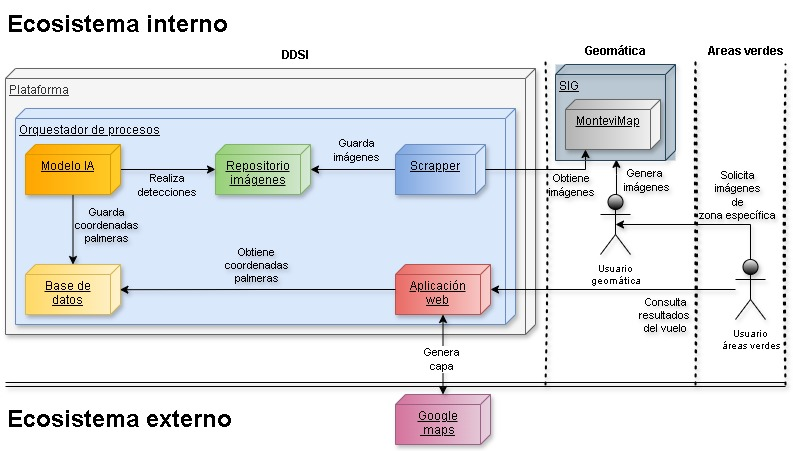
\includegraphics[width=.95\textwidth]{./Figuras/diagrama-inicial-solucion.jpg}
  \caption{Diagrama de la solución.}
  \label{fig:diagrama-inicial-solucion}
\end{figure}

La implementación de esta plataforma ofrece beneficios tanto económicos como ambientales para la IM. La detección temprana y tardía de la plaga puede reducir los costos de inspección presencial y optimizar el uso de drones, aprovechando su capacidad para cubrir grandes áreas. En particular, esta plataforma permitirá a la IM optimizar sus recursos en el manejo del picudo rojo, lo que reducirá los costos asociados a la remoción de palmeras, enfocará las inspecciones presenciales solo en casos excepcionales y permitirá la realización de vuelos programados de drones para maximizar su autonomía. Asimismo, validará un prototipo que puede extenderse a otros proyectos, que pueden contribuir a la preservación del entorno ecológico de la ciudad y a la seguridad de sus habitantes. Finalmente, se brinda la posibilidad de incorporar un módulo para la detección automática de palmeras en los vuelos aéreos.

\section{2. Identificación y análisis de los interesados}
\label{sec:interesados}

\begin{table}[ht]
  %\caption{Identificación de los interesados}
  %\label{tab:interesados}
  \begin{tabularx}{\linewidth}{@{}|l|X|X|l|@{}}
    \hline
    \rowcolor[HTML]{C0C0C0}
    Rol           & Nombre y Apellido        & Organización    & Puesto                        \\ \hline
    Cliente       & \clientename             & \empclientename & Director sector arbolado      \\ \hline
    Impulsor      & Msc. Ing. Juan Prada     & \empclientename & Gerente ciudades inteligentes \\ \hline
    Responsable   & \authorname              & \empclientename & Alumno                        \\ \hline
    Orientador    & \supname                 & \pertesupname   & Director del trabajo final    \\ \hline
    Usuario final & Usuarios de áreas verdes & \empclientename & Administrativo                \\ \hline
  \end{tabularx}
\end{table}

Descripción de los interesados:
\begin{itemize}
  \item Cliente: es experto en la problemática del picudo rojo y posee habilidades en gestión e implementación de soluciones diversas. Es uno de los principales promotores del proyecto y tiene un alto interés en su éxito.

  \item Impulsor: el Gerente de Ciudades Inteligentes cuenta con conocimientos sólidos tanto en inteligencia artificial como en gestión de proyectos. Es un impulsor clave de estas iniciativas, que se alinean con la visión estratégica de la organización.

  \item Orientador: el {\supname} tiene un conocimiento profundo en visión por computadora, particularmente en el contexto de esta problemática. Además, es profesor de {\pertesupname} en la asignatura de Visión por Computadora II, lo que le permite brindar apoyo técnico y conceptual al proyecto.

  \item Usuario final: los usuarios finales son técnicos de áreas verdes capacitados para identificar visualmente la plaga en las palmeras. Realizan el análisis de datos, gestionan la georreferenciación de las palmeras y, cuando es necesario, llevan a cabo inspecciones de campo.
\end{itemize}

\section{3. Propósito del proyecto}
\label{sec:proposito}

Proveer una prueba de concepto (POC) del componente de inteligencia artificial de una plataforma informática, alineada con la visión de la IM (\textit{Montevideo más verde}), que permita mejorar la eficiencia en la detección del \textit{Rhynchophorus ferrugineus}, utilizando técnicas avanzadas de visión por computadora y aprendizaje profundo.

\section{4. Alcance del proyecto}
\label{sec:alcance}

El alcance de la etapa inicial del proyecto incluye:
\begin{itemize}
  \item Investigar la viabilidad de la detección del \textit{Rhynchophorus ferrugineus} mediante técnicas de visión por computadora en dominios multiespectrales.
  \item Desarrollar un modelo de visión por computadora que permita detectar el \textit{Rhynchophorus ferrugineus} en palmeras de Montevideo.
  \item Gestionar el proceso de etiquetado de datos.
  \item Escribir una memoria con los resultados del proyecto.
\end{itemize}

En esta etapa, el proyecto no incluye:
\begin{itemize}
  \item La detección de la plaga y palmeras mediante imágenes de vuelos por aviones.
  \item Identificación del grado de infección de las palmeras, sino su clasificación binaria en infectadas y no infectadas.
  \item Otros componentes de la arquitectura presentada que no sea el modelo de visión por computadora.
  \item Las posibles extensiones de la plataforma.
  \item La gestión del ciclo de vida del modelo de detección.
  \item La evolución del sistema.
\end{itemize}

\section{5. Supuestos del proyecto}
\label{sec:supuestos}


Para el desarrollo del presente proyecto se supone que:

\begin{itemize}

  \item Se cuenta con disponibilidad horaria de al menos 20 horas semanales para realizar el proyecto.
  \item Se cuenta con imágenes de drones con resoluciones espaciales de al menos 3 cm/pixel.
  \item Se cuenta con voluntad del cliente para realizar el etiquetado de las imágenes.
  \item Se cuenta con la infraestructura necesaria para el despliegue de los componentes de software.
  \item Se cuenta con el apoyo de la IM para la ejecución del proyecto.
  \item Se cuenta con que se pueda detectar la plaga mediante imágenes RGB o infrarrojas (o combinación de ambas) obtenidas desde drones.
  \item Se cuenta con imágenes georeferenciadas.
  \item Se cuenta con mosaicos ortorectificados.

\end{itemize}

\section{6. Requerimientos}
\label{sec:requerimientos}

Para una mejor organización los requisitos se expresan utilizando una metodología de rotulado contextual, donde cada uno se identifica según su nivel de afinidad y jerárquico.

La notación se realiza en lenguaje natural, siguiendo un formato estandarizado, donde se especifica el actor y luego la funcionalidad.

La organización jerárquica se toma del template de referencia de especificación de requisitos de software de la IEEE \cite{SRSTemplateIEE}.

Finalmente, se priorizan utilizando el método \textit{MoSCoW} \cite{moscowMethod}.

\begin{enumerate}
  \item Requisitos de interfaces internas:
        \begin{enumerate}
          \item Modelo de visión por computadora
                \begin{enumerate}[label={[RII-ModeloVPC-\arabic*]}, leftmargin=*]
                  \item (S) El modelo de visión por computadora debe proporcionar un servicio web que reciba una imagen y devuelva una estructura de datos con las detecciones y sus coordenadas.
                \end{enumerate}
          \item Visualizador de detecciones
                \begin{enumerate}[label={[RII-VisDetecciones-\arabic*]}, leftmargin=*]
                  \item (S) El visualizador de detecciones debe aceptar una imagen y la estructura de datos de las detecciones, mostrando la imagen compuesta con las detecciones realizadas.
                \end{enumerate}
        \end{enumerate}

  \item Requisitos de interfaces externas:
        \begin{enumerate}
          \item Gestor de datos
                \begin{enumerate}[label={[RIF-GestorDatos-\arabic*]}, leftmargin=*]
                  \item (S) El gestor de datos debe ser accesible desde internet por los usuarios de áreas verdes.
                \end{enumerate}
          \item Visualizador de detecciones
                \begin{enumerate}[label={[RIF-VisDetecciones-\arabic*]}, leftmargin=*]
                  \item (S) El visualizador de detecciones debe ser accesible desde internet por los usuarios de áreas verdes.
                \end{enumerate}
        \end{enumerate}

  \item Requisitos funcionales:
        \begin{enumerate}
          \item Modelo de visión por computadora
                \begin{enumerate}[label={[RF-ModeloVPC-\arabic*]}, leftmargin=*]
                  \item (M) El modelo de visión debe ser capaz de generar predicciones a partir de una imagen proporcionada.
                  \item (M) El modelo de visión debe identificar palmeras en imágenes aéreas de forma precisa.
                  \item (M) El modelo de visión debe clasificar automáticamente las palmeras en dos categorías: infectadas y no infectadas.
                \end{enumerate}
          \item Visualizador de detecciones
                \begin{enumerate}[label={[RF-VisDetecciones-\arabic*]}, leftmargin=*]
                  \item (C) El visualizador de detecciones debe permitir la visualización de una imagen junto con sus detecciones.
                \end{enumerate}
          \item Gestor de datos
                \begin{enumerate}[label={[RF-GestorDatos-\arabic*]}, leftmargin=*]
                  \item (S) El gestor de datos debe incluir una herramienta para el etiquetado de datos que permita al cliente etiquetar imágenes de drones.
                  \item (C) El gestor de datos debe almacenar los datos etiquetados en el repositorio de la Intendencia Municipal (IMNube).
                \end{enumerate}
        \end{enumerate}

  \item Requisitos del proceso:
        \begin{enumerate}
          \item Modelo de visión por computadora
                \begin{enumerate}[label={[RP-ModeloVPC-\arabic*]}, leftmargin=*]
                  \item (S) Se debe investigar el estado del arte en modelos de visión por computadora para la detección de la plaga.
                  \item (C) Se debe realizar una investigación sobre enfoques de detección de plagas mediante imágenes multiespectrales.
                \end{enumerate}
          \item Gestor de datos
                \begin{enumerate}[label={[RP-GestorDatos-\arabic*]}, leftmargin=*]
                  \item (C) Se deben investigar herramientas adecuadas para el etiquetado de datos.
                \end{enumerate}
        \end{enumerate}

  \item Requisitos de datos:
        \begin{enumerate}
          \item Gestor de datos
                \begin{enumerate}[label={[RDATOS-GestorDatos-\arabic*]}, leftmargin=*]
                  \item (C) El sistema debe permitir al cliente etiquetar al menos 100 imágenes, asegurando un equilibrio entre las clases de palmeras infectadas y no infectadas.
                \end{enumerate}
        \end{enumerate}

  \item Requisitos de documentación:
        \begin{enumerate}
          \item Informe final
                \begin{enumerate}[label={[RDOC-InformeFinal-\arabic*]}, leftmargin=*]
                  \item (M) Se debe elaborar un informe final que incluya una presentación completa del proyecto y sus resultados.
                  \item (C) Se debe elaborar un informe de avance a mitad del tiempo asignado para el proyecto, detallando los progresos realizados.
                \end{enumerate}
        \end{enumerate}

  \item Requisitos de rendimiento:
        \begin{enumerate}
          \item Modelo de visión por computadora
                \begin{enumerate}[label={[RR-ModeloVPC-\arabic*]}, leftmargin=*]
                  \item (C) El modelo de visión por computadora debe mantener una precisión mínima del 90\% en la identificación de palmeras y un 80\% en la clasificación de infestación.
                  \item (C) El modelo de visión por computadora debe ser capaz de procesar imágenes capturadas en condiciones de iluminación variables.
                \end{enumerate}
        \end{enumerate}

  \item Requisitos de interfaces gráficas:
        \begin{enumerate}
          \item Visualizador de detecciones
                \begin{enumerate}[label={[RIG-VisDetecciones-\arabic*]}, leftmargin=*]
                  \item (C) El visualizador de detecciones debe brindar un criterio de satisfacción de usabilidad mayor al 80\% para los usuarios.
                \end{enumerate}
        \end{enumerate}

  \item Requisitos de seguridad (\textit{security}):
        \begin{enumerate}
          \item Gestor de datos
                \begin{enumerate}[label={[RS-GestorDatos-\arabic*]}, leftmargin=*]
                  \item (S) El gestor de datos debe estar bajo un mecanismo de autorización de usuarios.
                \end{enumerate}
          \item Visualizador de detecciones
                \begin{enumerate}[label={[RS-VisDetecciones-\arabic*]}, leftmargin=*]
                  \item (S) El visualizador de datos debe estar bajo un mecanismo de autorización de usuarios.
                \end{enumerate}
        \end{enumerate}

  \item Requisitos de diseño:
        \begin{enumerate}
          \item Lenguaje
                \begin{enumerate}[label={[RD-ModeloVPC-\arabic*]}, leftmargin=*]
                  \item (C) El sistema debe ser implementado utilizando \textit{Python 3} para el procesamiento backend.
                  \item (C) El sistema debe ser implementado utilizando \textit{Angular} para el procesamiento frontend.
                  \item (C) El protocolo de comunicación de los servicios debe ser \textit{REST}.
                \end{enumerate}
        \end{enumerate}
\end{enumerate}

\section{7. Historias de usuarios (\textit{Product backlog})}
\label{sec:backlog}

Las historias de usuario contienen sus criterios de aceptación, y se ponderan según la complejidad, dificultad e incertidumbre.
El resultado final de puntos de historia, es el número de \textit{Fibonacci} superior más cercano.

Los actores involucrados son:

\begin{table}[ht]
  \begin{tabularx}{\linewidth}{@{}|l|X|X|l|@{}}
    \hline
    \rowcolor[HTML]{C0C0C0}
    Actor                                & Descripción                                                                                                                                                             \\ \hline
    Usuario técnico de la IM             & El usuario técnico de la IM es el responsable de realizar la implementación técnica del proyecto, lo que incluye todo lo relacionado con el ciclo de vida del software. \\ \hline
    Usuario del servicio de áreas verdes & El usuario del servicio de áreas verdes es el encargado de interactuar con el software en modalidad de "usuario final".                                                 \\ \hline
    Usuario responsable del proyecto     & El usuario responsable del proyecto es el encargado en todas las disciplinas transversales del proyecto, como lo es la gestión, entre otros.                            \\ \hline
  \end{tabularx}
\end{table}

\begin{enumerate}
  \item Como usuario técnico de la IM quiero identificar palmeras en imágenes de drones ortorectificadas para detectar posibles casos de estudio de infestación.
        \begin{itemize}
          \item \textit{Story points}: 34 (complejidad: 8, dificultad: 8, incertidumbre: 13)
          \item Criterios de aceptación:
                \begin{itemize}
                  \item El sistema debe procesar imágenes y marcar las palmeras detectadas con sus respectivas coordenadas.
                  \item La detección debe mantener una precisión mínima del 90\%
                \end{itemize}
        \end{itemize}

  \item Como usuario técnico de la IM quiero clasificar las palmeras en imágenes de drones ortorectificadas en infectadas y no infectadas para detectar posibles casos de infestación.
        \begin{itemize}
          \item \textit{Story points}: 55 (complejidad: 13, dificultad: 13, incertidumbre: 13)
          \item Criterios de aceptación:
                \begin{itemize}
                  \item El sistema debe procesar imágenes con palmeras detectadas y marcar clasificarlas en infectadas o no infectadas.
                  \item El sistema debe mantener una precisión mínima del 80\% en el modelo de visión por computadora.
                \end{itemize}
        \end{itemize}

  \item Como usuario técnico de la IM quiero acceder e investigar información sobre el estado del arte en detección de plagas en dominios multiespectrales para asegurarme que el modelo de visión utilice los enfoques más efectivos.
        \begin{itemize}
          \item \textit{Story points}: 55 (complejidad: 21, dificultad: 13, incertidumbre: 8)
          \item Criterios de aceptación:
                \begin{itemize}
                  \item Se debe documentar una revisión de modelos de visión por computadora avanzados para la detección de plagas en el informe final.
                  \item La revisión debe incluir métodos actuales para detección en imágenes multiespectrales.
                  \item La revisión debe incluir casos de estudios de al menos dos modelos.
                \end{itemize}
        \end{itemize}

  \item Como usuario del servicio de áreas verdes quiero, dada una imagen, visualizar las palmeras que están infectadas o no para aplicar posibles tratamientos de la plaga.
        \begin{itemize}
          \item \textit{Story points}: 21 (complejidad: 8, dificultad: 5, incertidumbre: 8)
          \item Criterios de aceptación:
                \begin{itemize}
                  \item El sistema debe mostrar, dada una imagen proporcionada, cuales palmeras están infectadas y cuales no.
                  \item El sistema debe brindar una satisfacción de usabilidad mayor al 80\% en el visualizador de detecciones.
                \end{itemize}
        \end{itemize}

  \item Como usuario del servicio de áreas verdes quiero etiquetar las imágenes de los drones para brindarle al modelo de visión por computadora una mejor capacidad de predicción.
        \begin{itemize}
          \item \textit{Story points}: 21 (complejidad: 8, dificultad: 5, incertidumbre: 8)
          \item Criterios de aceptación:
                \begin{itemize}
                  \item El sistema debe proporcionar una herramienta que permita la selección y etiquetado de palmeras en imágenes de drones.
                  \item El sistema debe permitir el almacenamiento tanto de las imágenes sin etiquetar como las etiquetadas en la IMNube.
                  \item El sistema debe permitir que los usuarios accedan desde la internet al gestor de datos.
                \end{itemize}
        \end{itemize}

  \item Como usuario responsable del proyecto quiero que el sistema cuente con imágenes etiquetadas para asegurarme la robustez del modelo.
        \begin{itemize}
          \item \textit{Story points}: 89 (complejidad: 34, dificultad: 5, incertidumbre: 21)
          \item Criterios de aceptación:
                \begin{itemize}
                  \item Se debe etiquetar al menos 100 imágenes.
                  \item El etiquetado debe contener tanto la detección de la palmera como la clasificación en infectada y no infectada.
                \end{itemize}
        \end{itemize}

  \item Como usuario responsable del proyecto quiero el modelo de visión por computadora brinde una interfaz que permita consumir una imagen y exponer un servicio con las detecciones de dicha imagen para asegurarme de que el sistema sea escalable en otras iteraciones.
        \begin{itemize}
          \item \textit{Story points}: 21 (complejidad: 5, dificultad: 8, incertidumbre: 5)
          \item Criterios de aceptación:
                \begin{itemize}
                  \item El protocolo de comunicación debe ser \textit{REST}.
                \end{itemize}
        \end{itemize}

  \item Como usuario responsable del proyecto quiero acceder a un informe final con los resultados del proyecto para presentarlo ante los responsables de la IM y FIUBA.
        \begin{itemize}
          \item \textit{Story points}: 55 (complejidad: 34, dificultad: 5, incertidumbre: 5)
          \item Criterios de aceptación:
                \begin{itemize}
                  \item El informe final debe incluir la presentación completa del proyecto, resultados obtenidos y conclusiones.
                  \item Debe estar estructurado y listo para presentación en el formato provisto por la FIUBA.
                  \item Se debe presentar un informe de avance a la mitad del proceso.
                \end{itemize}
        \end{itemize}
\end{enumerate}

\section{8. Entregables principales del proyecto}
\label{sec:entregables}

Los entregables para esta etapa del proyecto son:

\begin{itemize}
  \item Aplicación para el etiquetado de datos.
  \item Aplicación para visualizar las detecciones.
  \item Modelo de visión por computadora.
  \item Código fuente referente a las aplicaciones.
  \item Informe final.
\end{itemize}

\section{9. Desglose del trabajo en tareas}
\label{sec:wbs}

\begin{enumerate}
  \item Análisis e investigación (100 h)
        \begin{enumerate}
          \item Análisis de tecnologías para el gestor de datos (20 h).
          \item Análisis de tecnologías para el visualizador de detecciones (20 h).
          \item Investigación del estado del arte en modelos de visión por computadora (30 h).
          \item Investigación específica para detección en imágenes multiespectrales (30 h).
        \end{enumerate}

  \item Diseño del sistema (50 h)
        \begin{enumerate}
          \item Diseño de arquitectura en general (10 h)
          \item Diseño de pruebas (5 h)
          \item Diseño del gestor de datos (5 h)
          \item Diseño del visualizador de detecciones (10 h)
          \item Diseño del modelo de visión por computadora (20 h)
        \end{enumerate}

  \item Construcción del sistema (180 h)
        \begin{enumerate}
          \item Construcción del sistema en general (20 h)
          \item Construcción del gestor de datos (40 h)
          \item Construcción del visualizador de detecciones (20 h)
          \item Construcción del modelo de visión por computadora (100 h)
                \begin{enumerate}[label*=\arabic*.]
                  \item Construcción del modelo (40 h)
                  \item Entrenamiento del modelo (40 h)
                  \item Adaptación del modelo (20 h)
                \end{enumerate}
        \end{enumerate}

  \item Validación y verificación del sistema (50 h)
        \begin{enumerate}
          \item Validación y verificación del gestor de datos (5 h)
          \item Validación y verificación del visualizador de detecciones (5 h)
          \item Validación y verificación del modelo de visión por computadora (30 h)
          \item Validación y verificación de la integración de aplicaciones (10 h)
        \end{enumerate}

  \item Implantación del sistema (50 h)
        \begin{enumerate}
          \item Configuración inicial (10 h)
          \item Implantación del gestor de datos (10 h)
          \item Implantación del visualizador de detecciones (10 h)
          \item Implantación del modelo de visión por computadora (20 h)
        \end{enumerate}

  \item Gestión del proyecto (50 h)
        \begin{enumerate}
          \item Planificación (10 h)
          \item Refinar planes (10 h)
          \item Versionado de herramientas, código y datos (10 h)
          \item Reuniones (10 h)
          \item Gestión del etiquetado de datos (10 h)
        \end{enumerate}

  \item Gestión de la documentación (120 h)
        \begin{enumerate}
          \item Escritura del informe de avance (20 h)
          \item Escritura memoria en taller de trabajo final A (40 h)
          \item Escritura memoria en taller de trabajo final B (40 h)
          \item Preparación de presentación del proyecto (20 h)
        \end{enumerate}

\end{enumerate}

Cantidad total de horas: 600 h

\section{10. Diagrama de Activity On Node}
\label{sec:AoN}

En la figura \ref{fig:AoN} se muestra el diagrama de precedencia de actividades. En color rojo, se muestra el camino crítico, que está definido por las siguientes tareas secuenciales:

$\rightarrow$ 1.3. Investigación del estado del arte en modelos de visión por computadora (30 h). \newline
$\rightarrow$ 1.4. Investigación específica para detección en imágenes multiespectrales (30 h). \newline
$\rightarrow$ 2.1. Diseño de arquitectura en general (10 h). \newline
$\rightarrow$ 2.5. Diseño del modelo de visión por computadora (20 h). \newline
$\rightarrow$ 3.1. Construcción del sistema en general (20 h). \newline
$\rightarrow$ 3.4.1. Construcción del modelo (40 h). \newline
$\rightarrow$ 3.4.1. Entrenamiento del modelo (40 h). \newline
$\rightarrow$ 3.4.1. Adaptación del modelo (20 h). \newline
$\rightarrow$ 4.3. Validación y verificación del modelo de visión por computadora (30 h). \newline
$\rightarrow$ 4.4. Validación y verificación de la integración de aplicaciones (10 h). \newline
$\rightarrow$ 5.1. Configuración inicial (10 h). \newline
$\rightarrow$ 5.4. Implantación del modelo de visión por computadora (20 h). \newline
$\rightarrow$ 7.1. Escritura del informe de avance (20 h). \newline
$\rightarrow$ 7.2. Escritura memoria en taller de trabajo final A (40 h). \newline
$\rightarrow$ 7.3. Escritura memoria en taller de trabajo final B (40 h). \newline
$\rightarrow$ 7.4. Preparación de presentación del proyecto (20 h). \newline


El camino crítico indica que el proyecto puede hacerse en un mínimo de 400 horas.

\begin{figure}[htpb]
  \centering
  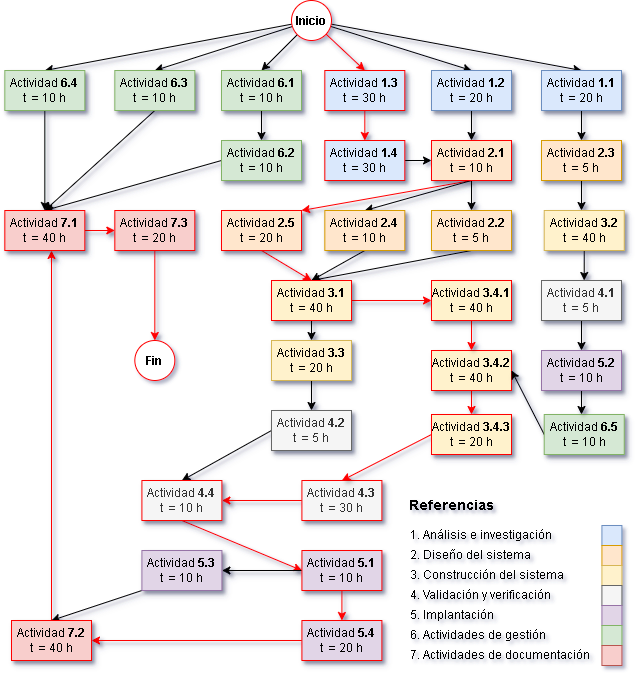
\includegraphics[width=.95\textwidth]{./Figuras/AoN.png}
  \caption{Diagrama de \textit{Activity on Node}.}
  \label{fig:AoN}
\end{figure}

\section{11. Diagrama de Gantt}
\label{sec:gantt}

En la figura \ref{fig:diagGanttAct} se puede observar la lista de actividades, y en la figura \ref{fig:diagGantt} el diagrama Gantt asociado a dicha lista.

\begin{figure}[htpb]
  \centering
  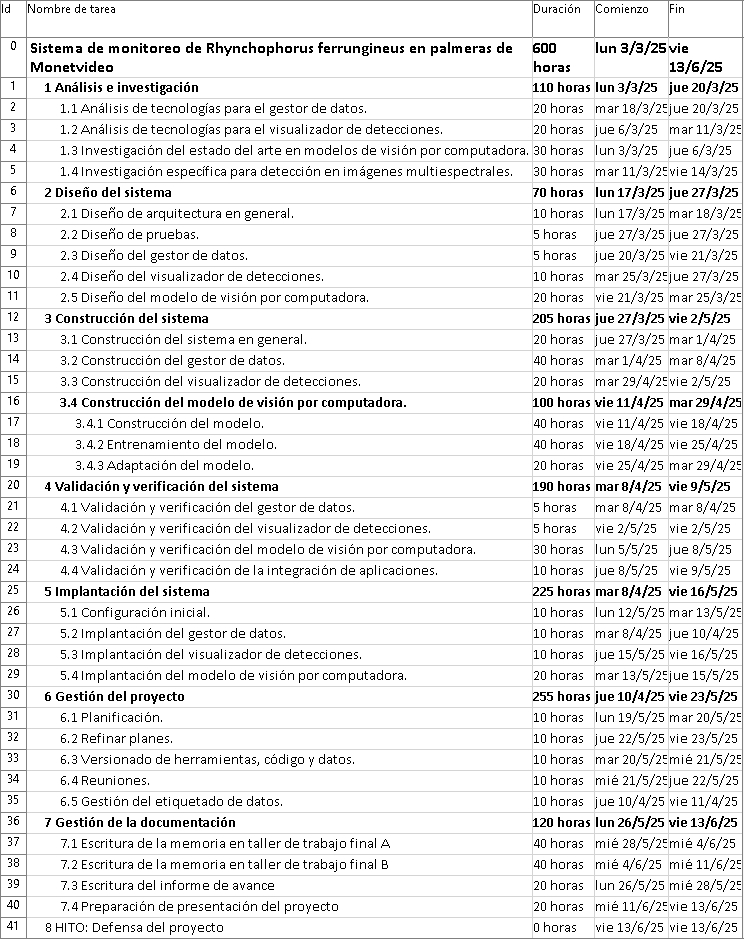
\includegraphics[height=.70\textheight]{./Figuras/lista-actividades.png}
  \caption{Lista de tareas para el Diagrama Gantt.}
  \label{fig:diagGanttAct}
\end{figure}

\begin{landscape}
  \centering
  \vspace*{\fill}
  \begin{figure}[htpb]
    \centering
    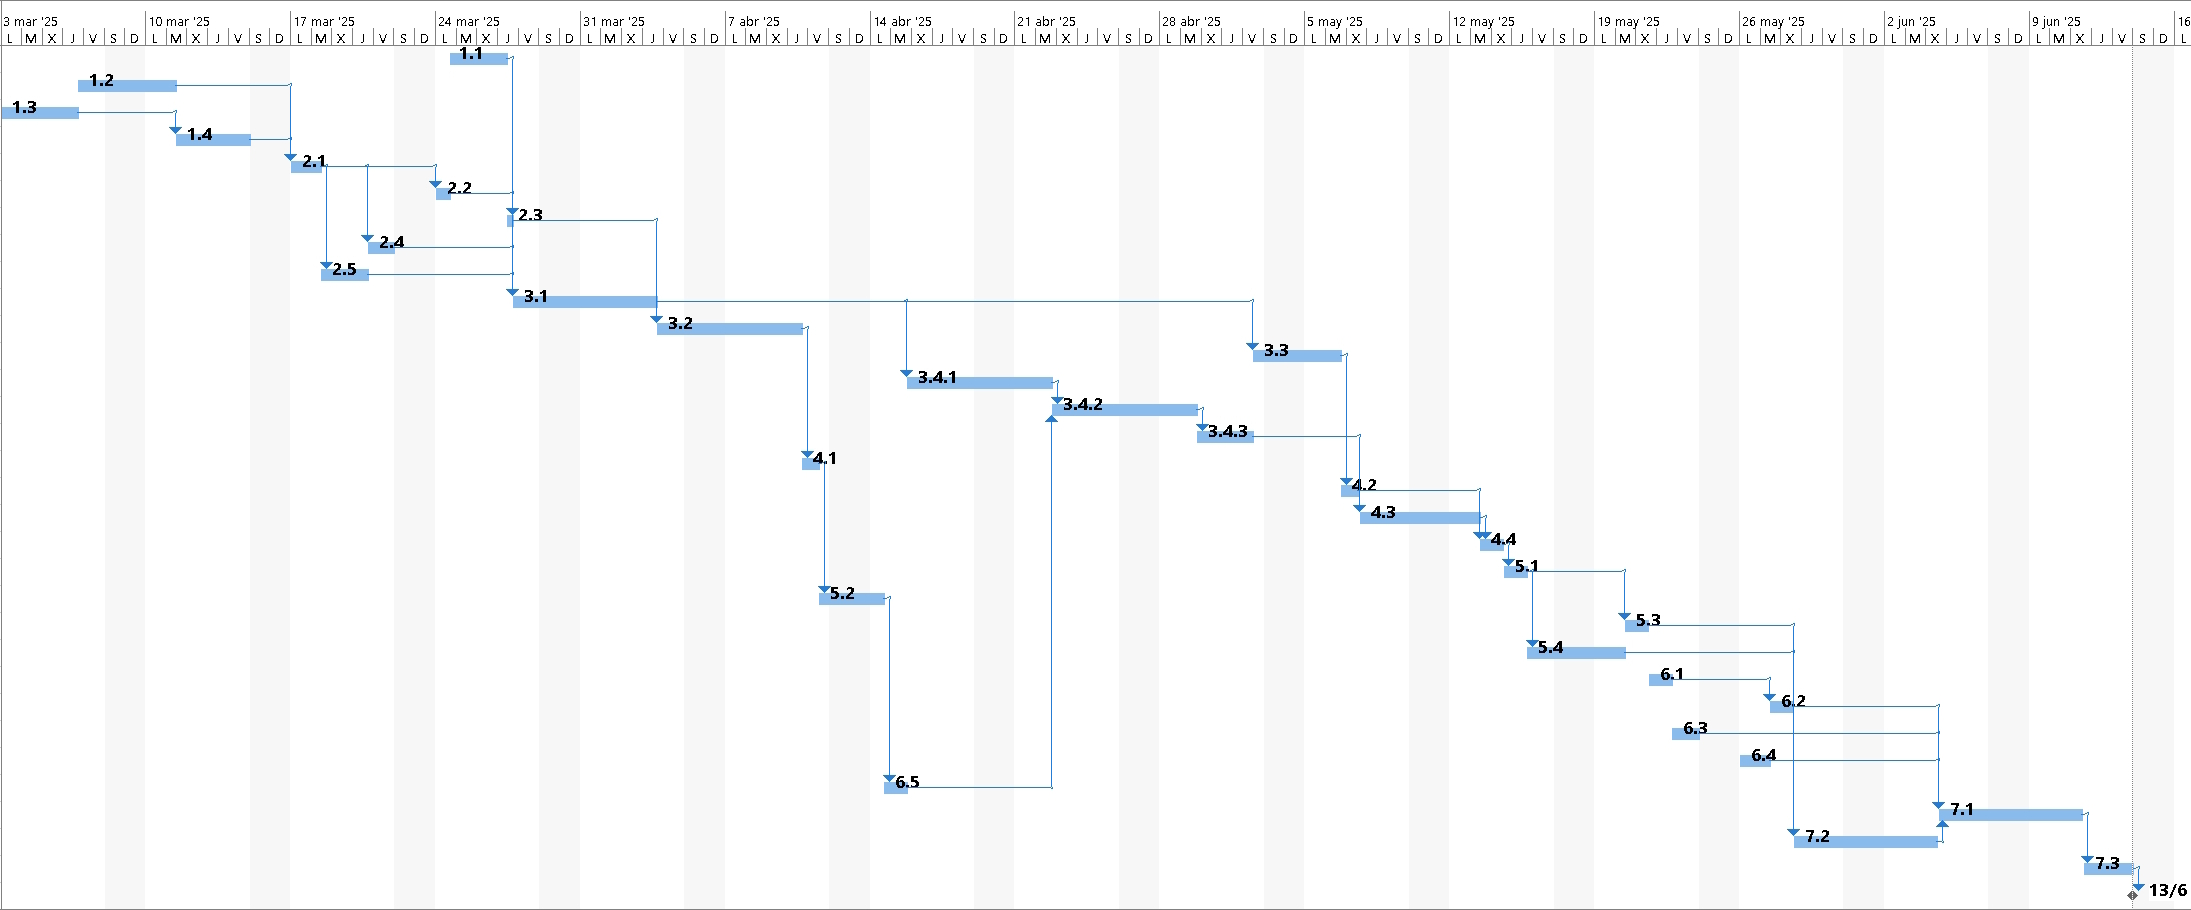
\includegraphics[height=.70\textheight]{./Figuras/gantt.jpg}
    \caption{Diagrama de Gantt.}
    \label{fig:diagGantt}
  \end{figure}
  \vfill
\end{landscape}


\section{12. Presupuesto detallado del proyecto}
\label{sec:presupuesto}

Los principales costos asociados de este proyecto se encuentran en las horas de ingeniería dedicadas. Como costos secundarios, las horas de personal cualificado para la realización del etiquetado de los datos. Como punto final, los datos ya se encuentran disponibles, sin embargo, es posible solicitarlos a demanda, por lo que estos costos también son incluidos.

\begin{table}[htpb]
  \centering
  \begin{tabularx}{\linewidth}{@{}|X|c|r|r|@{}}
    \hline
    \rowcolor[HTML]{C0C0C0}
    \multicolumn{4}{|c|}{\cellcolor[HTML]{C0C0C0}COSTOS DIRECTOS}   \\ \hline

    \rowcolor[HTML]{C0C0C0} Descripción                         &
    \multicolumn{1}{c|}{\cellcolor[HTML]{C0C0C0}Cantidad}       &
    \multicolumn{1}{c|}{\cellcolor[HTML]{C0C0C0}Valor unitario} &
    \multicolumn{1}{c|}{\cellcolor[HTML]{C0C0C0}Valor total}        \\ \hline

    Horas de ingeniería                                         &
    \multicolumn{1}{c|}{600 h}                                  &
    \multicolumn{1}{c|}{USD 30 / h}                             &
    \multicolumn{1}{c|}{USD 18000}                                  \\ \hline

    Horas de cómputo                                            &
    \multicolumn{1}{c|}{100 h}                                  &
    \multicolumn{1}{c|}{USD 0.1}                                &
    \multicolumn{1}{c|}{USD 10}                                     \\ \hline

    Infraestructura y almacenamiento                            &
    \multicolumn{1}{c|}{300 h}                                  &
    \multicolumn{1}{c|}{USD 0.1}                                &
    \multicolumn{1}{c|}{USD 30}                                     \\ \hline

    Horas de etiquetado                                         &
    \multicolumn{1}{c|}{40 h}                                   &
    \multicolumn{1}{c|}{USD 25}                                 &
    \multicolumn{1}{c|}{USD 1000}                                   \\ \hline

    Vuelos de drones                                            &
    \multicolumn{1}{c|}{5 U}                                    &
    \multicolumn{1}{c|}{USD 500}                                &
    \multicolumn{1}{c|}{USD 2500}                                   \\ \hline

    \multicolumn{3}{|c|}{SUBTOTAL}                              &
    \multicolumn{1}{c|}{USD 21540}                                  \\ \hline
    \rowcolor[HTML]{C0C0C0}
    \multicolumn{4}{|c|}{\cellcolor[HTML]{C0C0C0}COSTOS INDIRECTOS} \\ \hline

    \rowcolor[HTML]{C0C0C0} Descripción                         &
    \multicolumn{1}{c|}{\cellcolor[HTML]{C0C0C0}Cantidad}       &
    \multicolumn{1}{c|}{\cellcolor[HTML]{C0C0C0}Valor unitario} &
    \multicolumn{1}{c|}{\cellcolor[HTML]{C0C0C0}Valor total}        \\ \hline

    Imprevistos (40\% costos directos)                          &
    \multicolumn{1}{c|}{1 U}                                    &
    \multicolumn{1}{c|}{USD 8616}                               &
    \multicolumn{1}{c|}{USD 8616}                                   \\ \hline

    \multicolumn{3}{|c|}{SUBTOTAL}                              &
    \multicolumn{1}{c|}{USD 8616}                                   \\ \hline
    \rowcolor[HTML]{C0C0C0}
    \multicolumn{3}{|c|}{TOTAL}                                 &

    USD 30156                                                       \\ \hline
  \end{tabularx}%
\end{table}


\section{13. Gestión de riesgos}
\label{sec:riesgos}

En esta sección se identifican riesgos puntuales del proyecto, sus posibles mitigaciones y una matriz que permite observar los $RPN$ resultantes.

a) Identificación de los riesgos y estimación de sus consecuencias:

Riesgo 1: retrasos en el etiquetado de imágenes por parte del cliente.
\begin{itemize}
  \item Severidad ($S$): 8. El etiquetado de las imágenes es esencial para entrenar los modelos de aprendizaje profundo. Un retraso significativo podría comprometer los plazos del proyecto y la calidad de los resultados. \item Probabilidad de ocurrencia ($O$): 6. Aunque el cliente muestra voluntad, la tarea de etiquetado puede ser más demandante de lo inicialmente previsto, afectando su disponibilidad.
\end{itemize}

Riesgo 2: limitaciones en la calidad de las imágenes capturadas por los drones.
\begin{itemize}
  \item Severidad ($S$): 9. La calidad de las imágenes (resolución espacial, georreferenciación, ausencia de ruido) es crítica para la detección precisa de la plaga. Imágenes de baja calidad dificultarían el entrenamiento y la inferencia del modelo.
  \item Probabilidad de ocurrencia ($O$): 5. Aunque se cuenta con imágenes de alta resolución, factores como las condiciones climáticas o fallos técnicos en los drones podrían afectar su calidad.
\end{itemize}

Riesgo 3: limitaciones en la infraestructura para el procesamiento de datos.
\begin{itemize}
  \item Severidad ($S$): 7. El procesamiento de imágenes y el entrenamiento de modelos requieren infraestructura computacional robusta. Limitaciones en esta área podrían generar cuellos de botella.
  \item Probabilidad de ocurrencia ($O$): 4. Se supone que la infraestructura necesaria está disponible, pero problemas de configuración o recursos insuficientes podrían surgir durante el proyecto.
\end{itemize}

Riesgo 4: dificultades para detectar la plaga mediante las imágenes disponibles.
\begin{itemize}
  \item Severidad ($S$): 10. Si las imágenes (RGB, infrarrojas o combinadas) no permiten identificar de manera confiable la plaga, el objetivo principal del proyecto estaría en riesgo.
  \item Probabilidad de ocurrencia ($O$): 5. Estudios previos sugieren que estas técnicas son viables, pero no se puede descartar que ciertas características de la plaga sean difíciles de detectar en las condiciones del entorno, principalmente aquellas características que permitan una detección temprana.
\end{itemize}

Riesgo 5: pérdida de apoyo por parte de la IM.
\begin{itemize}
  \item Severidad ($S$): 8. La IM es un actor clave para el éxito del proyecto, tanto en términos de apoyo logístico como en la visión estratégica. Su pérdida implicaría una reestructuración importante.
  \item Probabilidad de ocurrencia ($O$): 2. Hasta ahora, la IM ha mostrado disposición, pero eventos políticos o administrativos podrían modificar su nivel de apoyo.
\end{itemize}

Riesgo 6: errores en la georreferenciación de las imágenes.
\begin{itemize}
  \item Severidad ($S$): 8. La georreferenciación precisa es esencial para analizar la distribución espacial de la plaga y para generar mapas de acción. Errores en esta etapa pueden comprometer la utilidad del sistema final.
  \item Probabilidad de ocurrencia ($O$): 3. Aunque las imágenes se supone que están georreferenciadas, problemas técnicos durante la captura o el procesamiento pueden introducir errores. Sin embargo, la IM cuenta con infraestructura y \textit{software} especial para trabajar con información geográfica.
\end{itemize}

Riesgo 7: falta de representatividad en el conjunto de datos.
\begin{itemize}
  \item Severidad ($S$): 9. Si el conjunto de datos no incluye suficientes ejemplos de las condiciones reales del entorno (iluminación, vegetación, diferentes estados de infestación), el modelo podría tener un bajo desempeño en escenarios reales.
  \item Probabilidad de ocurrencia ($O$): 6. La recopilación de datos representativos puede ser difícil debido a la variabilidad de las condiciones ambientales y la distribución de la plaga.
\end{itemize}

Riesgo 8: escalabilidad limitada del sistema.
\begin{itemize}
  \item Severidad ($S$): 7. Si el sistema no puede manejar un volumen creciente de imágenes o áreas a analizar, su utilidad para el cliente será limitada.
  \item Probabilidad de ocurrencia ($O$): 4. Esto dependerá de la eficiencia de la implementación del sistema, así como de la infraestructura disponible en ese momento.
\end{itemize}

Riesgo 9: problemas legales o de privacidad relacionados con el uso de drones.
\begin{itemize}
  \item Severidad ($S$): 8. Restricciones legales o preocupaciones de privacidad sobre el uso de drones pueden limitar las áreas en las que se permite la captura de imágenes.
  \item Probabilidad de ocurrencia ($O$): 2. Aunque se supone que se cuenta con apoyo de la IM, los permisos específicos para ciertos vuelos podrían enfrentar retrasos o restricciones imprevistas.
\end{itemize}

Riesgo 10: sobreajuste del modelo a los datos de entrenamiento.
\begin{itemize}
  \item Severidad ($S$): 6. Si el modelo se adapta demasiado a los datos de entrenamiento, su capacidad para generalizar a nuevas imágenes será limitada, afectando su utilidad en el campo.
  \item Probabilidad de ocurrencia ($O$): 6. Es un riesgo inherente en proyectos de aprendizaje profundo, pero puede mitigarse con técnicas adecuadas de regularización y validación.
\end{itemize}

Riesgo 11: cambios en las prioridades del cliente.
\begin{itemize}
  \item Severidad ($S$): 6. Si el cliente modifica las prioridades del proyecto, los objetivos iniciales podrían ser redefinidos, generando retrabajos o desviaciones en el cronograma.
  \item Probabilidad de ocurrencia ($O$): 2. Aunque se cuenta con apoyo inicial del cliente, factores externos o cambios internos en su organización podrían alterar sus prioridades.
\end{itemize}

Riesgo 12: Insuficiencia de imágenes etiquetadas.
\begin{itemize}
  \item Severidad ($S$): 8. Un número insuficiente de imágenes etiquetadas reduce la capacidad del modelo para generalizar, afectando su precisión y desempeño.
  \item Probabilidad de ocurrencia ($O$): 6. El etiquetado es una tarea laboriosa y puede no completarse en el tiempo previsto.
\end{itemize}

b) Tabla de gestión de riesgos (el $RPN$ se calcula como $RPN=S*O$):

\begin{table}[H]
  \centering
  \begin{tabularx}{\linewidth}{@{}|X|c|c|c|c|c|c|@{}}
    \hline
    \rowcolor[HTML]{C0C0C0}
    Riesgo                                                                   & $S$ & $O$ & $RPN$ & $S^*$ & $O^*$ & $RPN^*$ \\ \hline
    1. Retrasos en el etiquetado de imágenes por parte del cliente           & 8   & 6   & 48    & 8     & 3     & 24      \\ \hline
    2. Limitaciones en la calidad de las imágenes capturadas por los drones  & 9   & 5   & 45    & 6     & 2     & 12      \\ \hline
    3. Limitaciones en la infraestructura para el procesamiento de datos     & 7   & 4   & 28    & -     & -     & -       \\ \hline
    4. Dificultades para detectar la plaga mediante las imágenes disponibles & 10  & 5   & 50    & 10    & 3     & 30      \\ \hline
    5. Pérdida de apoyo por parte de la IM                                   & 8   & 2   & 16    & -     & -     & -       \\ \hline
    6. Errores en la georreferenciación de las imágenes                      & 8   & 3   & 24    & -     & -     & -       \\ \hline
    7. Falta de representatividad en el conjunto de datos                    & 9   & 6   & 54    & 8     & 3     & 24      \\ \hline
    8. Escalabilidad limitada del sistema                                    & 7   & 4   & 28    & -     & -     & -       \\ \hline
    9. Problemas legales o de privacidad relacionados con el uso de drones   & 8   & 2   & 16    & -     & -     & -       \\ \hline
    10. Sobreajuste del modelo a los datos de entrenamiento                  & 6   & 6   & 36    & 5     & 2     & 10      \\ \hline
    11. Cambios en las prioridades del cliente                               & 6   & 2   & 12    & -     & -     & -       \\ \hline
    12. Insuficiencia de imágenes etiquetadas                                & 8   & 6   & 48    & 7     & 3     & 21      \\ \hline
  \end{tabularx}%
  \caption{Matriz de riesgos del proyecto.}
\end{table}

Como criterio adoptado para la mitigación de los riesgos, se tomarán medidas donde los números de $RPN$ sean mayores a 30.

Nota: los valores marcados con ($^*$) en la tabla corresponden luego de haber aplicado la mitigación.

c) Plan de mitigación de los riesgos que originalmente excedían el $RPN$ máximo establecido:

Riesgo 1: retrasos en el etiquetado de imágenes por parte del cliente.
\begin{itemize}
  \item Plan de mitigación: implementar un sistema de etiquetado semiautomático utilizando algoritmos de visión por computadora para reducir la carga de trabajo manual, aprovechando la información geográfica disponible (es posible detectar palmeras mediante aprendizaje por transferencia y luego utilizando la ubicación clasificarlas como infectadas o no). Además, establecer hitos intermedios para monitorear el avance del etiquetado y ofrecer apoyo al cliente.
  \item Nueva asignación de $S$ y $O$ ($S^*$, $O^*$):
        \begin{itemize}
          \item Severidad ($S^*$): 8. La severidad se mantiene, ya que el etiquetado sigue siendo esencial para el proyecto.
          \item Probabilidad de ocurrencia ($O^*$): 3. Con el sistema semiautomático y la supervisión del progreso, la probabilidad de retrasos disminuye significativamente.
        \end{itemize}
\end{itemize}

Riesgo 2: limitaciones en la calidad de las imágenes capturadas por los drones.
\begin{itemize}
  \item Plan de mitigación: establecer protocolos para revisar la calidad de las imágenes inmediatamente después de la captura. En caso de problemas, se realizarán vuelos adicionales en las áreas afectadas. Además, preparar algoritmos que puedan manejar ciertas imperfecciones en las imágenes.
  \item Nueva asignación de $S^*$ y $O^*$:
        \begin{itemize}
          \item Severidad ($S^*$): 6. La severidad se reduce, ya que el impacto de imágenes de baja calidad puede ser mitigado parcialmente con algoritmos robustos, así como una buena comunicación con el Departamento de Geomática.
          \item Probabilidad de ocurrencia ($O^*$): 2. Con los protocolos de control de calidad y la posibilidad de vuelos adicionales, es menos probable que las imágenes finales sean inadecuadas.
        \end{itemize}
\end{itemize}

Riesgo 4: dificultades para detectar la plaga mediante las imágenes disponibles.
\begin{itemize}
  \item Plan de mitigación: utilizar enfoques actuales del estado del arte, que incluyen modelos de última generación como \textit{vision transformers}.
  \item Nueva asignación de $S^*$ y $O^*$:
        \begin{itemize}
          \item Severidad ($S^*$): 10. Se mantiene la severidad, ya que el objetivo del proyecto depende de una buena detección de la plaga.
          \item Probabilidad de ocurrencia ($O^*$): 3. Utilizando modelos y técnicas de última generación, aumenta la posibilidad de detectar la plaga.
        \end{itemize}
\end{itemize}

Riesgo 7: falta de representatividad en el conjunto de datos.
\begin{itemize}
  \item Plan de mitigación: asegurar la diversidad del conjunto de datos recopilando imágenes de diferentes zonas, condiciones climáticas y estados de infestación. Además, utilizar técnicas de aumento de datos (\textit{data augmentation}) para simular escenarios diversos.
  \item Nueva asignación de $S^*$ y $O^*$:
        \begin{itemize}
          \item Severidad ($S^*$): 8. Aunque el impacto sigue siendo alto, la representatividad se mejora significativamente con un conjunto de datos diverso y técnicas de aumento. \item Probabilidad de ocurrencia ($O^*$): 3. Con un enfoque proactivo en la recopilación de datos y el uso de \textit{data augmentation}, se reduce la probabilidad de falta de representatividad. \end{itemize}
\end{itemize}

Riesgo 10: sobreajuste del modelo a los datos de entrenamiento.
\begin{itemize}
  \item Plan de mitigación: aplicar regularización adecuada (\textit{Dropout}, \textit{L2}) y realizar una validación cruzada exhaustiva para garantizar la generalización del modelo. Incorporar nuevos datos en el entrenamiento si es posible.
  \item Nueva asignación de $S^*$ y $O^*$:
        \begin{itemize}
          \item Severidad ($S^*$): 5. Con una adecuada validación y regularización, el impacto del sobreajuste disminuye significativamente.
          \item Probabilidad de ocurrencia ($O^*$): 2. La probabilidad se reduce drásticamente con las técnicas mencionadas, asegurando un modelo más generalizable.
        \end{itemize}
\end{itemize}

Riesgo 12: insuficiencia de imágenes etiquetadas.
\begin{itemize}
  \item Plan de mitigación: ampliar el equipo encargado del etiquetado para incluir colaboradores adicionales en caso de necesidad. Además, priorizar el etiquetado de las áreas más críticas y utilizar técnicas de aprendizaje semisupervisado para trabajar con datos parcialmente etiquetados.
  \item Nueva asignación de $S^*$ y $O^*$:
        \begin{itemize}
          \item Severidad ($S^*$): 7. Aunque sigue siendo crítico, el impacto se reduce al priorizar áreas clave y utilizar técnicas semisupervisadas.
          \item Probabilidad de ocurrencia ($O^*$): 3. Con un equipo ampliado y estrategias adicionales, la probabilidad de insuficiencia de datos etiquetados se reduce significativamente.
        \end{itemize}
\end{itemize}

\section{14. Gestión de la calidad}
\label{sec:calidad}

La gestión de la calidad de incluye actividades de conformidad y no conformidad con los diez requerimientos más importantes:
\begin{itemize}[label={}]
  \item {[}RF-ModeloVPC-3{]} El modelo de visión debe clasificar automáticamente las palmeras en dos categorías: infectadas y no infectadas.
        \begin{itemize}
          \item Verificación:
                \begin{itemize}
                  \item Implementar un conjunto de pruebas unitarias con imágenes previamente etiquetadas para medir la precisión del modelo en la clasificación.
                  \item Realizar una prueba de estrés con al menos 100 imágenes con distintas condiciones de iluminación y perspectivas.
                  \item Revisar los resultados comparándolos con las etiquetas originales y asegurar que la tasa de clasificación correcta sea al menos 80\%.
                \end{itemize}
          \item Validación:
                \begin{itemize}
                  \item Presentar un informe al cliente con las métricas de clasificación obtenidas, incluyendo precisión, \textit{recall} y \textit{F1-score}.
                  \item Organizar una demostración con el cliente donde pueda verificar los resultados usando imágenes propias.
                \end{itemize}
        \end{itemize}

  \item {[}RII-ModeloVPC-1{]} El modelo de visión por computadora debe proporcionar un servicio web que reciba una imagen y devuelva una estructura de datos con las detecciones y sus coordenadas.
        \begin{itemize}
          \item Verificación:
                \begin{itemize}
                  \item Realizar pruebas unitarias con solicitudes HTTP simuladas para verificar que el servicio web responde correctamente.
                  \item Inspeccionar que la estructura de datos devuelta sea conforme al formato especificado (\textit{JSON} con coordenadas precisas).
                  \item Revisar los logs del servidor para garantizar que no existen errores o tiempos de respuesta excesivos.
                \end{itemize}
          \item Validación:
                \begin{itemize}
                  \item Proporcionar al cliente una herramienta que permita enviar imágenes y recibir resultados, verificando que los resultados son útiles y correctos según su criterio.
                  \item Realizar una sesión con el cliente para probar el servicio con casos reales.
                \end{itemize}
        \end{itemize}

  \item {[}RF-VisDetecciones-1{]} El visualizador de detecciones debe permitir la visualización de una imagen junto con sus detecciones.
        \begin{itemize}
          \item Verificación:
                \begin{itemize}
                  \item Probar el sistema con diferentes conjuntos de imágenes para garantizar que las detecciones se muestran correctamente sobre las imágenes originales.
                  \item Evaluar que los \textit{bounding boxes} son precisos y corresponden a las coordenadas devueltas por el modelo.
                \end{itemize}
          \item Validación:
                \begin{itemize}
                  \item Realizar una sesión con el cliente para mostrar el funcionamiento del visualizador con imágenes reales y recibir retroalimentación sobre la presentación de los resultados.
                  \item Proveer una interfaz al cliente para probar el visualizador con sus propias imágenes.
                \end{itemize}
        \end{itemize}

  \item {[}RR-ModeloVPC-1{]} El modelo de visión por computadora debe mantener una precisión mínima del 90\% en la identificación de palmeras y un 80\% en la clasificación de infestación.
        \begin{itemize}
          \item Verificación:
                \begin{itemize}
                  \item Entrenar el modelo utilizando un conjunto de validación y evaluar las métricas de desempeño (precisión y \textit{recall}).
                  \item Documentar los resultados con gráficos \textit{ROC} y matrices de confusión para cada categoría.
                \end{itemize}
          \item Validación:
                \begin{itemize}
                  \item Presentar al cliente los resultados obtenidos y explicar las métricas en términos no técnicos.
                \end{itemize}
        \end{itemize}

  \item {[}RDATOS-GestorDatos-1{]} El sistema debe permitir al cliente etiquetar al menos 100 imágenes, asegurando un equilibrio entre las clases de palmeras infectadas y no infectadas.
        \begin{itemize}
          \item Verificación:
                \begin{itemize}
                  \item Probar la herramienta de etiquetado asegurando que puede cargar, procesar y guardar imágenes etiquetadas sin errores.
                  \item Realizar pruebas con imágenes de cada clase para garantizar el equilibrio en los datos generados.
                  \item Ejecutar pruebas de integración entre la herramienta y la infraestructura (base de datos).
                  \item Realizar una prueba para verificar que la herramienta esté accesible desde internet.
                \end{itemize}
          \item Validación:
                \begin{itemize}
                  \item Organizar una sesión con el cliente para utilizar la herramienta y verificar que puede etiquetar imágenes de forma intuitiva y eficiente.
                  \item Solicitar retroalimentación directa del cliente para ajustes.
                \end{itemize}
        \end{itemize}

  \item {[}RP-ModeloVPC-1{]} Se debe investigar el estado del arte en modelos de visión por computadora para la detección de la plaga.
        \begin{itemize}
          \item Verificación:
                \begin{itemize}
                  \item Documentar los modelos investigados, incluyendo sus métricas de desempeño y posibles adaptaciones para el proyecto.
                  \item Comparar los resultados obtenidos con los modelos seleccionados para justificar la elección final.
                \end{itemize}
          \item Validación:
                \begin{itemize}
                  \item Revisar el documento de investigación con el cliente y explicar cómo las decisiones tomadas benefician al proyecto.
                  \item Confirmar que el cliente está de acuerdo con la elección del modelo.
                \end{itemize}
        \end{itemize}

  \item {[}RF-GestorDatos-2{]} El gestor de datos debe almacenar los datos etiquetados en el repositorio de la Intendencia Municipal (IMNube).
        \begin{itemize}
          \item Verificación:
                \begin{itemize}
                  \item Realizar pruebas automatizadas para verificar la conexión al repositorio y la correcta subida de los datos etiquetados.
                  \item Revisar manualmente que los datos almacenados están completos y accesibles.
                \end{itemize}
          \item Validación:
                \begin{itemize}
                  \item Confirmar que el cliente puede acceder a los datos según lo esperado.
                \end{itemize}
        \end{itemize}

  \item {[}RD-ModeloVPC-1{]} El sistema debe ser implementado utilizando Python 3 para el procesamiento backend.
        \begin{itemize}
          \item Verificación:
                \begin{itemize}
                  \item Inspeccionar los archivos fuente para garantizar que cumplen con la especificación.
                  \item Realizar auditorías de código para verificar que las librerías utilizadas son compatibles con Python 3.
                \end{itemize}
          \item Validación:
                \begin{itemize}
                  \item Proporcionar al cliente evidencia de que el sistema se ejecuta correctamente en entornos configurados con Python 3.
                \end{itemize}
        \end{itemize}

  \item {[}RII-VisDetecciones-1{]} El visualizador de detecciones debe brindar un criterio de satisfacción de usabilidad mayor al 80\% para los usuarios.
        \begin{itemize}
          \item Verificación:
                \begin{itemize}
                  \item Realizar pruebas de usabilidad con un grupo piloto, registrando tiempos de interacción y número de errores.
                  \item Documentar las métricas obtenidas y compararlas contra el objetivo establecido.
                \end{itemize}
          \item Validación:
                \begin{itemize}
                  \item Organizar una sesión de prueba con el cliente y usuarios finales para recibir retroalimentación sobre la usabilidad del sistema.
                  \item Ajustar el sistema si la satisfacción está por debajo del 80\%.
                \end{itemize}
        \end{itemize}

  \item {[}RF-GestorDatos-1{]} El gestor de datos debe incluir una herramienta para el etiquetado de datos que permita al cliente etiquetar imágenes de drones.
        \begin{itemize}
          \item Verificación:
                \begin{itemize}
                  \item Probar exhaustivamente la herramienta asegurando que las funcionalidades básicas (carga de imágenes, etiquetado, guardado) funcionan correctamente.
                  \item Simular escenarios de uso para detectar posibles errores.
                \end{itemize}
          \item Validación:
                \begin{itemize}
                  \item Entrenar al cliente en el uso de la herramienta y recopilar retroalimentación después de una sesión práctica.
                  \item Realizar ajustes según sea necesario para cumplir con las expectativas del cliente.
                \end{itemize}
        \end{itemize}

  \item {[}RDOC-InformeFinal-1{]} Se debe elaborar un informe final que incluya una presentación completa del proyecto y sus resultados.
        \begin{itemize}
          \item Verificación:
                \begin{itemize}
                  \item Revisar el informe final asegurando que cumple con los siguientes aspectos:
                        \begin{itemize}
                          \item Explicación detallada del objetivo del proyecto.
                          \item Descripción de la metodología utilizada, incluyendo los modelos seleccionados y su entrenamiento.
                          \item Análisis de los resultados obtenidos, con métricas claras y gráficos representativos.
                          \item Conclusiones y recomendaciones futuras.
                          \item Asegurar que la estructura sea la proporciona por la \pertesupname.
                          \item Verificar que el informe esté estructurado y redactado en un lenguaje claro y profesional.
                        \end{itemize}
                \end{itemize}
          \item Validación:
                \begin{itemize}
                  \item Entregar el informe final a los interesados y realizar una presentación del contenido.
                \end{itemize}
        \end{itemize}
\end{itemize}

\section{15. Procesos de cierre}
\label{sec:cierre}

Dentro de los procesos de cierre de este proyecto se llevarán a cabo las siguientes actividades:

\begin{itemize}
  \item Realización de un análisis comparativo entre el plan inicial y la ejecución real, destacando desviaciones, logros y áreas de mejora.
  \item Evaluación de los procedimientos, técnicas aplicadas y los principales desafíos enfrentados durante el ciclo de vida del proyecto.
  \item Elaboración de propuestas concretas de mejora para futuros proyectos similares, basadas en las lecciones aprendidas.
  \item Presentación de los resultados y entregables del proyecto a los interesados de la Intendencia de Montevideo.
  \item Organización de una defensa formal del proyecto en el marco de la Facultad de Ingeniería de la Universidad de Buenos Aires, con la participación de los principales interesados.
  \item Consolidación y archivo de toda la documentación relevante en los repositorios institucionales de la IM y de la FIUBA, garantizando su accesibilidad y conservación.
\end{itemize}

\bibliographystyle{unsrt} % Estilo de la bibliografía.
\bibliography{charter} % Nombre del archivo .bib sin extensión

\end{document}